\documentclass[]{article}
\usepackage[utf8]{inputenc}
\usepackage[margin=1.0in]{geometry}
\usepackage{amsmath, amsfonts}
\usepackage{tikz}
\usepackage[english]{babel}
\usepackage{amsthm}
\usepackage{enumitem}
\usepackage{graphicx}
\usepackage{fancyhdr}
\usepackage{subcaption}
\usepackage{float}

\newcommand{\bd}{\textbf}

\pagestyle{fancy}
\fancyhf{}
\title{Confirming Bragg's Law using X-Ray Diffraction from an NaCl Crystal}
\author{Kale Stahl}
\lhead{X-Ray Diffraction from an NaCl Crystal}
\rhead{Kale Stahl}

\begin{document}
	
	\maketitle
	\begin{abstract}
		
	\end{abstract}
	\section{Introduction}
		The arrangement of atoms or ions in crystals can be understood as an array of parallel lattice. These lattices will form planes in which waves can be scattered, creating a spherical wavelet. In this situation, our wavelength $\lambda$ of the incident wagve is unchanged and 
		
		Bragg's law states that the glancing angle $\theta$ is related to an integer multiple of the incident wavelength $\lambda$ in the following way
		\begin{equation}
			n\lambda = 2d\sin \theta \label{bragg's law}
		\end{equation}
		In essence, this means that with a fixed $\lambda$ there exists some $\theta$ that depends on $d$, the distance between objects in the lattice, in which we have that the angle of incidence is equal to the angle of reflection.
		
	\section{Experimental Procedure}
		\subsection{Apparatus}
		We will use the Lehr-und Didaktiksysteme X-ray Apparatus 554 800 with serial number . A visualization of this apparatus is seen in Figure \ref{apparatus}. This apparatus is equipped with a built in X-ray tube, goniometer, and Geiger-M\"uller counter, We will detail the exact specifications and use of each of these components below.
		\begin{figure}[h!]
			\begin{center}
				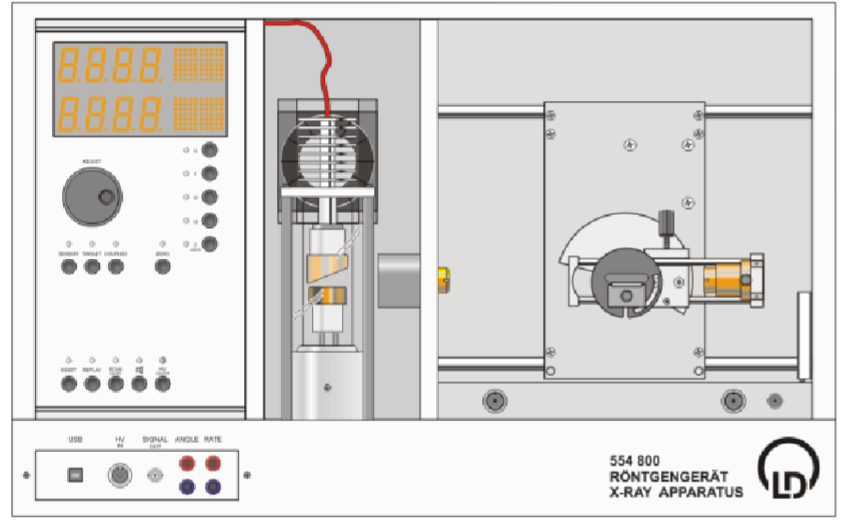
\includegraphics[width = .45\textwidth]{apparatus}
			\end{center}
			\caption{Visualization of the Lehr-und Didaktiksysteme X-ray Apparatus 554 800}
			\label{apparatus}
		\end{figure}
		\subsubsection*{X-Ray Tube}
			The X-ray tube uses a molybdenum anode in a copper block whose purpose is to dissipate heat. This molybdenum has $K_\alpha = 17.4$ keV and $K_\beta = 19.6$ keV.
			\begin{figure}[h!]
				\begin{subfigure}{.45\textwidth}
					\begin{center}
						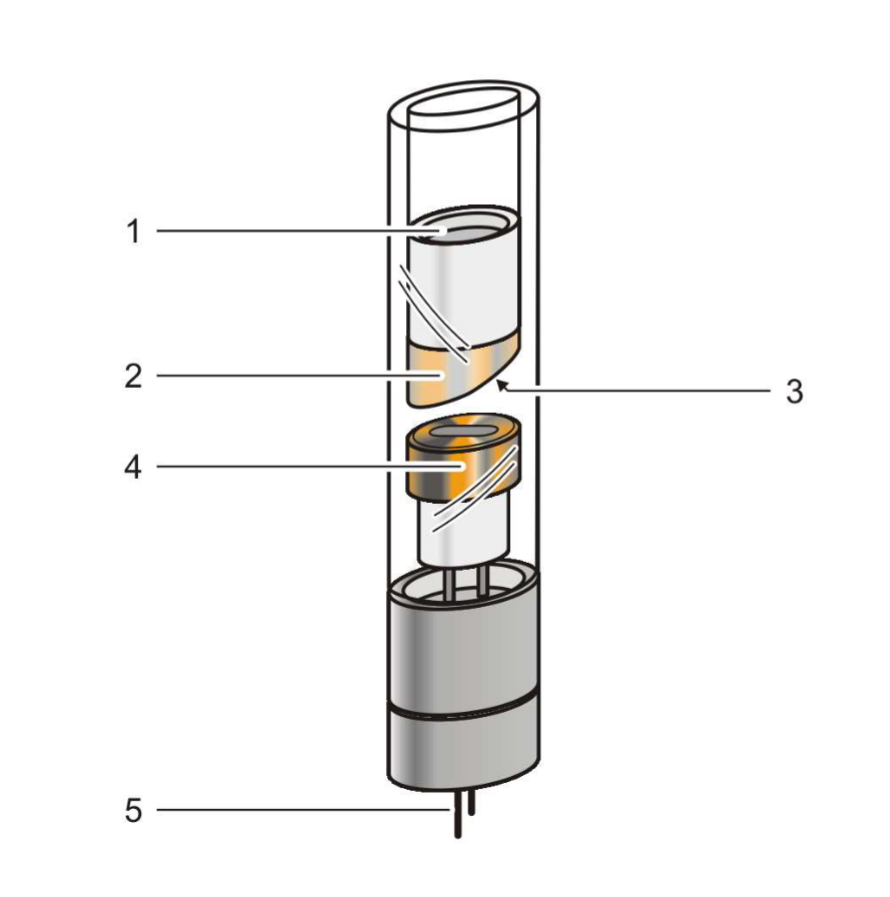
\includegraphics[width = .5\textwidth]{x-ray tube}
					\end{center}
					\caption{Labeled visualization of the x-ray tube. Numbered components are as follows: \bd{(1)} Thread for heat sink; \bd{(2)} Copper block; \bd{(3)} Molybdenum anode; \bd{(4)} Hot cathode; \bd{(5)} Pin socket Base }
					\label{x-ray tube}
				\end{subfigure}
				\hspace{.05\textwidth}
				\begin{subfigure}{.45\textwidth}
					\begin{center}
						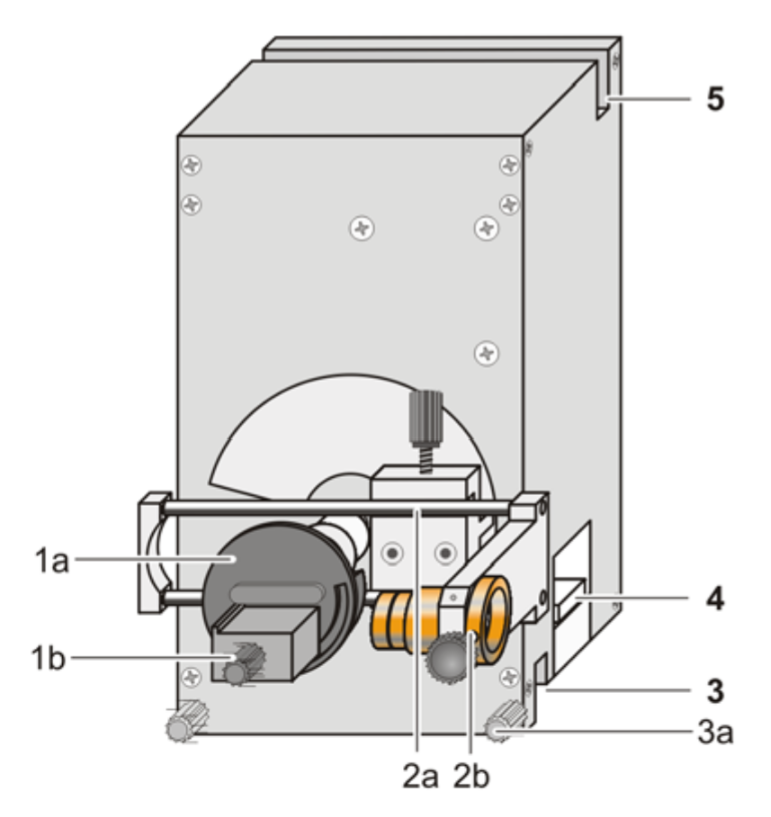
\includegraphics[width = .5\textwidth]{goniometer}
					\end{center}
					\caption{Labeled visualization of the goniometer. Numbered components are as follows: \bd{(1)} Target arm; \bd{(2)} Sensor arm; \bd{(3)} Bottom guide groove; \bd{(4)} Terminal pin connector; \bd{(5)} Top guide groove }
					\label{goniometer}
				\end{subfigure}
				\caption{Descriptions of x-ray tube and goniometer}
			\end{figure}
		\subsubsection*{Goniometer}
			This goniometer is a self-contained unit for mounting the crystal sample and the detector. It is internally calibrated so that the GM Counter will move twice the angle of the sample for each rotation in order to maintain the Bragg angle. The goniometer has unlimited angle range with an angular resolution of $0.1^\circ$.
		\subsubsection*{Geiger-M\"uller Counter}
			We will utilize a self-quenching Geiger-M\"uller counter with a thin mica window $d = 12- 15$ mm with a filling of neon, argon, and halogen gas. This will be used to detect the x-ray radiation scattering off the crystal. It has an energy range of greater than 2.5 keV for x-ray radiation.
		\subsubsection*{NaCl Crystal}
			The NaCl crystal we will use is a 25 by 25 by 4 millimeter NaCl crystal with the spacing of lattice planes being 282 pm. This crystal has theoretical reflection angles of $7.24^\circ$ for $K_\alpha$ and $6.43^\circ$ for $K_\beta$ from the molybdenum x-ray tube.
		\subsection{Data Collection}
	
	\section{Data Analysis}
	
	\section{Results and Conclusions}
	
	\newpage
	\section*{References}
	
\end{document}